\documentclass[a4paper,14pt]{article}
% \\ новая строка , cases - фигурная скобка
%substack друг под другом пишет
\usepackage[T2A]{fontenc}        
\usepackage[utf8]{inputenc}   
\usepackage[russian]{babel}

\usepackage[left=25mm, right=15mm, top=20mm, bottom=20mm]{geometry} 

\usepackage{graphicx}

\usepackage{amsmath}
\usepackage{amssymb} 

\usepackage{fancyhdr}
\usepackage[hidelinks]{hyperref}
\usepackage{cite}
\usepackage{amsthm}

\usepackage{verbatim}

\usepackage{multirow} 

\newtheorem{definition}{Определение}
\newtheorem{task}{Задача}

\pagestyle{fancy}   
\fancyhf{}          

\fancyhead[C]{\thepage}   
\fancyfoot[R]{\today}     
\renewcommand{\headrulewidth}{0pt}

\begin{document}

\tableofcontents
\newpage

\setcounter{equation}{47}

\section{Пределы}

\cite{art1}

\subsection{Предел последовательности}


\begin{equation}
\lim_{n \to \infty}\frac{\sqrt[3]{n^2}\sin n}{n+1}
\end{equation}

\setcounter{equation}{144}

\begin{equation}
\lim_{n \to \infty} \left(\frac{1^p+3^p+\dots+n^p}{n^p}-\frac{n}{p+1}\right)=\frac{1}{2}, \quad p\in\mathbb{N}
\end{equation}

\setcounter{equation}{631}

\begin {equation}
\lim_{n \to \infty}\sum\limits_{k=1}^{n} \left(\sqrt[3]{1+\frac{k}{n^2}}-1\right)
\end{equation}


\subsection{Предел функции}

\setcounter{equation}{624}

\begin{equation}
\lim_{n \to \infty} \frac{ x\tan^{2n}\frac{\pi x}{4}}{\tan^{2n}\frac{\pi x}{4} + 1}
\end{equation}

\setcounter{equation}{1342}
\begin{equation}
\lim_{x \to 0} x^{x^{x}-1}
\end{equation}

\setcounter{equation}{1369}
\begin{equation}
\lim_{x \to +\infty} \left[ \left(x+a\right)^{1+\frac{1}{x}} - x^{1+\frac{1}{x+a}}\right]
\end{equation}

\section{Интегралы}
\subsection{Неопределенные интегралы}

\setcounter{equation}{0}

\begin{equation}
\int \frac{1}{\sqrt{x^2\pm a^2}} \, dx = \ln{|x+\sqrt{x^2 \pm a^2}|}+ C,  \quad (a>0)
\end{equation}

\begin{equation}
\int \sqrt{a^2-x^2} \, dx = \frac{x}{2}\sqrt{a^2-x^2}+ \frac{a^2}{2}\arcsin \frac{x}{a} +C, \quad (a>0)
\end{equation}

\setcounter{equation}{1782}

\begin{equation}
\int x\sqrt{\frac{x}{2a-x}} \, dx
\end{equation}

\subsection{Определенные интегралы}

\setcounter{equation}{2237}

\begin{equation}
\int\limits_{0}^{\pi} \frac{\sin^2 x}{\sqrt{1-2\alpha\cos x +\alpha^2}} \,dx
\end{equation}

\setcounter{equation}{2273}
\begin{equation}
\int\limits_{0}^{3} \arcsin \sqrt{\frac{x}{1+x}} \,dx
\end{equation}

\setcounter{equation}{2283}
\begin{equation}
\int\limits_{0}^{2\pi} e^{inx}e^{-imx} \,dx = 
\begin{cases}
0, &  если m \ne n \\ 
2\pi, & если m = n
\end{cases}
\end{equation}

\setcounter{equation}{2356}

\subsection{Несобственные интегралы}
\begin{equation}
\lim_{x \to \infty} \dfrac{\int\limits_{0}^{x} \sqrt{1+t^4} \,dt}{x^3}
\end{equation}

\setcounter{equation}{2356}

\begin{equation}
\lim_{x \to 0} \dfrac{\int\limits_{x}^{+\infty} t^{-1} e^{-t} \,dt}{\ln{\frac{1}{x}}}
\end{equation}

\setcounter{equation}{2374}
\begin{equation}
\int\limits_{e}^{+\infty} \dfrac{1}{x^p \left(\ln x\right)^q \left(\ln\ln x\right)^r} \,dx
\end{equation}

\subsection{Двойные интегралы}

\setcounter{equation}{3947}
\begin{equation}
\int\limits_{-\frac{\pi}{2}}^{\frac{\pi}{2}} \, d\varphi \int\limits_{0}^{a\cos \varphi} f(\varphi,r) \, dr \quad (a>0)
\end{equation}

\setcounter{equation}{3951}
\begin{equation}
\iint\limits_{\Omega} f(\sqrt{x^2+y^2}) \,dx\,dy , \quad где \Omega =\{|y| \le |x| ; |x| \le 1\}
\end{equation}

\setcounter{equation}{3970}
\begin{equation}
\iint\limits_{\substack{0 \le x \le \pi \\ 0 \le y \le \pi}} |\cos (x+y)|\,dx\,dy
\end{equation}

\begin{equation}
\iint\limits_{x^2+y^2 \le 1} \left| \frac{x+y}{\sqrt{2}} - x^2 -y^2\right| \,dx\,dy
\end{equation}

\setcounter{equation}{3978}
\begin{equation}
\iint\limits_{\substack{0\le x \le t \\ 0\le y \le t}} e^{\frac{tx}{y^2}} \,dx\,dy
\end{equation}

\subsection{Тройные интегралы}

\setcounter{equation}{4095}
\begin{equation}
\iiint\limits_{x^2+y^2+z^2 \le R^2} \frac{\,dx\,dy\,dz}{\sqrt{(x-a)^2+(y-b)^2+(z-c)^2}},  \quad a^2+b^2+c^2 > R
\end{equation}

\subsubsection{Приложение тройных интегралов к механике}

\setcounter{equation}{0}
\begin{equation}
X= G\frac{\partial u}{\partial x} =G \iiint\limits_{V} \rho \dfrac{\xi - x}{r^3} \,d\xi \,d\eta \,d\zeta
\end{equation}

\subsection{Несобственные тройные интегралы}

\setcounter{equation}{4193}

\begin{equation}
\int\limits_{0}^{a}\int\limits_{0}^{a}\int\limits_{0}^{a} \dfrac{f(x,y,z) \,dx\,dy\,dz}{\{ [y -\varphi(x)]^{2} \} - \{ [z-\psi (x)]^{2}\}^p}
\end{equation}

\section{Ряды}

\subsection{Знакопеременные ряды}

\setcounter{equation}{2677}
\begin{equation}
\sum\limits_{n=1}^{\infty} \left(-1\right)^{n-1} \frac{2^n \sin^{2n} x}{2}
\end{equation}

\setcounter{equation}{2680}
\begin{equation}
\sum\limits_{n=1}^{\infty} \frac{\left(-1\right)^{n-1}}{\left[ \sqrt{n}+\left(-1\right)^{n-1}\right]^p}
\end{equation}

\setcounter{equation}{2683}
\begin{equation}
\sum\limits_{n=1}^{\infty} \left(-1\right)^{\frac{n\left(n-1\right)}{2}} \frac{n^{100}}{2^n}
\end{equation}

\subsection{Функциональные ряды}

\setcounter{equation}{2794}
\begin{equation}
f(x)=\sum\limits_{n=1}^{\infty} \dfrac{x}{(1+x^2)^n}
\end{equation}

\setcounter{equation}{2797}

\begin{equation}
\theta(x)=\sum\limits_{n=-\infty}^{+\infty} e^{-\pi n^2 x}
\end{equation}

\setcounter{equation}{2805}

\begin{equation}
\lim_{x \to 1-0} \sum\limits_{n=1}^{\infty} \dfrac{(-1)^ {n+1} }{n} \cdot \frac{x^n}{x^n+1}
\end{equation}



\subsection{Степенные ряды}

\setcounter{equation}{2823}

\begin{equation}
\sum\limits_{n=1}^{\infty}\dfrac{3^{-\sqrt{n}}x^{n}}{\sqrt{n^2+1}}
\end{equation}

\setcounter{equation}{2825}

\begin{equation}
\sum\limits_{n=1}^{\infty} \dfrac{(-1)^n}{n!} \left(\dfrac{e}{n}\right)^n x^n
\end{equation}

\setcounter{equation}{2829}

\begin{equation}
\sum\limits_{n=2}^{\infty}\dfrac{\left( 1+2\cos \dfrac{\pi n}{4} \right)^n }{\ln n} x^n
\end{equation}

\setcounter{equation}{2833}

\begin{equation}
\sum\limits_{n=1}^{\infty} \dfrac{1}{x^n} \sin \frac{\pi}{2^n}
\end{equation}

\setcounter{equation}{2836}

\begin{equation}
\sum\limits_{n=1}^{\infty}\dfrac{3^{3n}\left(n!\right)^3}{\left( 3n \right)!} \tan ^n x
\end{equation}

\subsubsection{Ряд Тейлора}
\begin{definition}
Ряд Тейлора 
\label{def:taylor}
\[ 
f(x) = \sum\limits_{k=0}^{\infty} \frac{f^{(k)} \left(a\right)}{k!} \left(x-a\right)^k
\]
Остаточный член ряда 
\[
R_n(x)=f(x) -  \sum\limits_{k=0}^{n} \frac{f^{(k)} \left(a\right)}{k!} \left(x-a\right)^k
\]
может быть представлен в виде 
\[
R_n(x)=\dfrac{f^{(n+1)}\left(a+\theta\left(x-a\right)\right)}{\left(n+1\right)!} \left(x-a\right)^{n+1} \quad (0<\theta<1)
\]
(форма Лагранжа) или в виде
\[
R_n(x)=\dfrac{f^{(n+1)}\left(a+\theta_1\left(x-a\right)\right)}{n!} \left( 1- \theta_1\right) ^n \left( x-a\right)^{n+1} \quad (0<\theta_1<1)
\]
(форма Коши)
\end{definition}

\begin{task}
Используя монотонность производных \(f^{(n)} (x)\) для остаточного члена \(R_n(x)\) ряда Тейлора (см. определение~\ref{def:taylor}) функции \(f(x)\),получить оценку
\[
|R_n(x)| \le |x|^{n+1}f(1)
\]
\end{task}

\section{Уравнения поверхностей}
 
\cite{art2}
 
\subsection{Уравнения}
\setcounter{equation}{4120}

\begin{equation}
\left( \frac{x^2}{a^2} + \frac{y^2}{b^2} +\frac{z^2}{c^2} \right) ^{2} = \frac{z}{h} \cdot e^{\frac{\frac{z^2}{c^2}}{\frac{x^2}{a^2}+\frac{y^2}{b^2}+\frac{z^2}{c^2}}}
\end{equation}

\begin{equation}
\frac{\frac{x}{a}+\frac{y}{b}}{\frac{x}{a}+\frac{y}{b}+\frac{z}{c}}=\frac{2}{\pi} \arcsin( \frac{x}{a}+\frac{y}{b}+\frac{z}{c} )
\end{equation}

\setcounter{equation}{4128}

\begin{equation}
\left( \frac{x^2}{a^2} + \frac{y^2}{b^2} \right) ^{n} + \frac{z^{2n}}{c^{2n}} = \frac{z}{h} \left( \frac{x^2}{a^2} +\frac{y^2}{b^2} \right)^{n-2} \quad (n>1).
\end{equation}

\setcounter{equation}{0}
\begin{equation}
z=x^2-y^2 \quad \text{(См.рисунок~\ref{fig:paraboloid})}
\end{equation}

\newpage

\subsection{График}

\begin{figure}[!h]
\centering
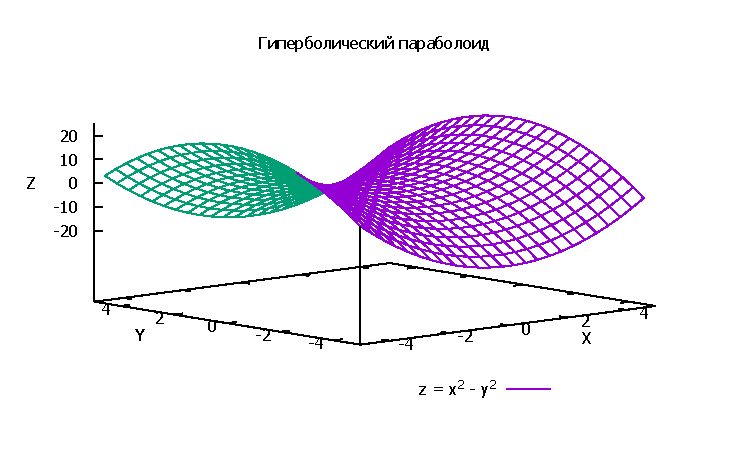
\includegraphics[width=0.8\textwidth]{./ris/pr1.pdf}
\caption{Гиперболический параболоид}
\label{fig:paraboloid}
\end{figure}

\newpage

\section{Таблица}

\begin{table}[h]
\centering
\begin{tabular}{|c|c|c|}
\hline
\multicolumn{3}{|c|}{Заголовок} \\
\hline
\multirow{2}{*}{A} & B & C \\
\cline{2-3}
& D & E \\
\hline
F & G & H \\
\hline
\end{tabular}
\caption{Таблица}
\label{tab}
\end{table}

См. таблицу~\ref{tab}

\clearpage
\phantomsection
\addcontentsline{toc}{section}{Список литературы}

\begin{thebibliography}{99}
\bibitem{art1} Демидович Б.\,П. Сборник задач и упражнений по математическому анализу.
\bibitem{art2} А.\,П. Комбаров, Ю.\,В. Садовничий. Аналитическая геометрия. 
\end{thebibliography}

\end{document}